\chapter[A$\beta$42]{Molecular Mechanism of A$\beta$42 fibril inhibition by inositol}
% Some notes
% I found these pretty neat ref articles on sciencedirect
% http://www.sciencedirect.com.myaccess.library.utoronto.ca/science/article/pii/B9780444519672001550
% http://www.sciencedirect.com.myaccess.library.utoronto.ca/science/article/pii/B9780444519672000581
% http://www.sciencedirect.com.myaccess.library.utoronto.ca/science/article/pii/B9780444519672000313
% http://www.sciencedirect.com.myaccess.library.utoronto.ca/science/article/pii/B0080437486011592

\section{Summary}
	Alzheimer's disease (AD) is a severe neurodegenerative disease with no cure. Currently, one method of targeting the underlying disease is to prevent or reverse the amyloid formation of A$\beta$42, a key pathological hallmark of AD. A small-molecule novel drug candidate, Scyllo-inositol, is a polyol small-molecule that exhibits stereochemistry dependent inhibition of the formation of fibrils in vitro.  Furthermore, recently completed phase II clinical trials demonstrated that scyllo-inositol achieved target drug levels in the cerebral spinal fluid (CSF) of AD patients, a main challenge for AD drug candidates to to overcome.
	Despite its promise as a therapeutic for AD, the mechanism of action of scyllo-inositol at the molecular level is currently not understood.  We perform extensive atomistic molecular dynamics simulations of scyllo-inositol and its inactive stereoisomer, chiro-inositol, glucose, and the osmolyte protein stabilizer, glycerol, with the full length A$\beta$42 protofibril.  From our simulations, we characterize the stereochemistry-dependent binding modes of these three cosolutes on the structure of A$\beta$42 protofibrils.  Our results provide molecular insight for the rational design of small-molecule inhibitors of A$\beta$42 and other amyloid-based diseases.

  \textbf{Keywords}:
	amyloid computational
	amyloid inhibition
	small molecule amyloid inhibition
	amyloid disaggregation
	inositol
	surface binding
	weak interactions
	carbohydrate like interactions

\section{Introduction}

\ab42 is the pathological hallmark of Alzheimer's Disease (AD) and forms the largest component of plaques deposits found in the brain of AD patients.\cite{Selkoe:1991uc} \ab42 is cleaved from amyloid precursor protein (APP) and are produced as peptides with lengths from 39 to 42 residues.   In vitro, \ab42 is found to aggregate much faster than \ab40\cite{Jarrett:1993vm,Fukumoto:1996vi,Finder:2010jw}, and are also found to form fibrils through distinct pathways.\cite{Bitan:2003ut,Sanchez:2011bj,Bitan:2003gx}  Furthermore, \ab42 much more toxic than \ab40 in both cell cultures\cite{ElAgnaf:2000hp} and animal models.\cite{Mucke:2000uq}

Although the ultrastructure of amyloid fibrils are often similar, typically they exhibit polymorphism where structural details are sequence-specific.\cite{Wu:2010p3553} Furthermore, there are differences in the fibril structures of \ab42 and \ab40.\cite{Ahmed:2010p5694}  Solid state NMR fibril models of \ab40 show that there can be 2 or 3 layers.\cite{Wu:2010p3553} A recent SSNMR model of the \ab42\cite{Tycko:2010iz}. The N-terminus of \ab42 peptides in fibrils was unstructured.\cite{Ahmed:2010p5694} Fibril structures of \ab40 and \ab42 were also found to be similar.\cite{Wu:2010p3553} There are brain derived structures of \ab40, their structures are different from the synthetic ones because of polymorphism. Different amyloid fibril structures may exhibit different toxicities.\cite{Paravastu:2009fi,Wu:2010p3553}

% rationale for studying the Abeta42 protofibril system	
Less information is known about the structures of non-fibrillar oligomers of \ab42. However, recent experimental studies suggest that toxicity oligomers may have cross-$\beta$ like structural elements.\cite{Stroud:2012dp} Previous MD simulations of \ab42 protofibrils\cite{Masman:2009p6410} suggests that 17-42 are responsible for the stability of the fibril.
	
% Small molecules are promising candidates for the treatment of AD. 

Furthermore, osmolytes such as carbohydrates, for example, trehalose\cite{Liu:2005km} and glycerol\cite{Sukenik:2011jf} have been shown to modulate amyloid formation and peptide aggregation REF Glycerol is able to slow the kinetics of fibrillation (I don't think this is correct). REF

Small-molecule modulators of amyloid formation may be classified into those that accelerate and / or stabilize amyloid formation and those that displace the equilibrium towards the disaggregated state (inhibitors of amyloid formation). Inositol is a polyhydroxylated compound that have been demonstrated to act on \ab42 with a stereochemistry-dependent activity. In mice studies, it [FILL IN THE BLANK HERE]. Our previous study of inositol binding to A$\beta$(16-22) suggests that inositol preferentially binds more ordered $\beta$-oligomers over small disordered aggregates.

In a previous study, our results indicate that inositol preferentially bind to surfaces of $\beta$-oligomers, but not to disordered or monomeric forms of A$\beta$(16-22).  Furthermore, binding modes are sequence-dependence of binding, the equilibrium binding constants for (GA)$_4$ was XX mM compared to ~5mM for the protofibrillar aggregate of A$\beta$(16-22). In this study, we examine the binding mechanism of inositol stereoisomers, and in addition, inactive compounds glucose and glycerol, with the full length NMR structure of Abeta42.  Both glucose and glycerol are known to be inactive in preventing the fibrillation of A$\beta$42. Our results provide into the structure-activity relationship of inositol in the inhibition of A$\beta$ amyloid formation, and advances our understanding towards a pharmcophore for treating Alzheimer's Disease.

%%%%%%%%%
Here we review the following recent simulation studies 

Simulations of binding to disordered peptides are computationally challenging.  Heterogeneous disordered peptides are a challenge because of the difficulty in obtaining convergence of their equilibrium ensemble of structures.  We've only seen a few of these studies carried out - there was one with A$\beta$ by Garcia et al. But I think that was it. 

To unambiguously determine the effect of a single small molecule's effect on the aggregation pathway of a peptide such as A$\beta$ requires microseconds of sampling per state, and at the same time comparatively studying the aggregation equilibrium of the peptide in absence of this small molecule.

Ideally, one should collectively examine the inhibitor of interest with different aggregate species in tandem with a system with which we can also observe the aggregation equilibrium of the peptide. 

We have done this with inositol with many different morphologies of different peptides and all of these systems collectively to draw on a possible molecular mechanism by a small molecule inhibitor.

http://www.jbc.org/content/286/48/41578.short

Simulations thus far which have examined small molecule binding with peptides that are truncated (such as that of A$\beta$(12-28) and A$\beta(16-22)$) forms of the full-length peptides of Abeta (AD) or alpha synuclein or IAPP. If not the the shorter peptide, studies typically employed forms with structure such as  the protofibril of Abeta40 or Abeta42 both of which have SSNMR starting structure coordinates.

In 2007, Duan et al. performed short simulation studies of the protofibrils of IAPP in the presence of four molecules of congo red. The study examined congo red binding with IAPP protofibrils, where they found that congo red predominantly adopted two binding modes: either along the group of the fibril or parallel to each of the peptide strands.  
In 2012, Congo red binding was examined with protofibrils of A$\beta$(1-40). http://www.cell.com/biophysj/abstract/S0006-3495(12)00780-1
Another early study of 9,10-Antrhaquinone suggests that intercalation and interactions between the backbone of peptides destabilize oligomer formation. http://onlinelibrary.wiley.com/doi/10.1002/pro.87/full

In 2010, Lemkul et al. used another short simulation study to examine binding of morin molecules with the protofibril form of abeta42.  They saw that they make hydrogen bonds and they concluded that studies with different forms of abeta42 is needed because small molecules may interact with any of the species in the aggregation pathway.

Molecular mechanism of ThT binding was probed in recent years by several simulation studies. Shea 2011 attempts to study the difference in binding between PIB and ThT.  Simulation of a ThT-based molecule with a charged group, another was the unmodified ThT molecule.  They were both seen to binding at the tunnel of the fibril. http://www.cell.com/biophysj/abstract/S0006-3495(11)00143-3

EGCG, a small molecule that is thought to inhibit aggregation of both alpha-synuclein and abeta42 by interacting with the monomer was also a popular system.  A study by wang 2010 showed that it adopted dual binding mode depending on the stoichiometry of the EGCG.
It was later shown that the prominent interaction comes form nonpolar binding in this study http://www.ncbi.nlm.nih.gov/pubmed/21899367 -- Liu FF study.

Ibuprofen and Naproxen, molecules which show demonstrated in vitro activity as an amyloid inhibitor was also probed using molecular simulations. In that study,  replica exchange was used to probe binding of both molecules with the protofibril of Abeta40 (the ssnmr structure).  results indicate that they might bind in grooves at the edges of the oligomers, which is a possible way by which it may prevent fibril formation. and that they bound predominantly via hydrophobic interactions.  

% Garcia et al. studied
At the time of writing, recent studies of anti-amyloid agents in literature includes galantamine
Some docking studies were also done. For more detail on this, see the recent review by Lemkul et al. http://www.ncbi.nlm.nih.gov/pubmed/23200245



%%%%%%%%%%




% Summary of Duan et al.\cite{Li:2011ei}
% \begin{itemize}
% 	\item Abeta42 monomer in helix conformation (pdb code: 1Z0Q)
% 	\item Abeta42 fibril (pdb code: 2BEG) - unmodified pentamer from the NMR structure	
% 	\item unrestrained MD. 80 ns per system, 4 replicas (for both monomer and fibril systems).  Only last 20 ns was used. AMBER FF03 force field
% \end{itemize}
% 
% Summary of Ahmed et al.\cite{Ahmed:2010p5694}
% \begin{itemize}
% 	\item Experimental. Conditions at low temperature 4 C and low salt conditioins (5 -10 mM)
% 	\item Attempt to characterize prefibrillar aggregates of Abeta42. Unlike Abeta42 fibrils, these neurotoxic oligomers do not form parallel, in-register beta-sheets. Also looked at the fibril structure of Abeta42 and found it was not consistent with Luhr’s et al model, but rather more similar to the Abeta40 model (Tycko et al)
% \end{itemize}

% Table template for entering simulation times
% \begin{table}\footnotesize
%   \begin{center}
%   \vspace{10pt}
%   \caption{Summary of simulation systems}
%   \label{tbl:simulations}
%     \begin{tabular}{| p{3cm} | *{7}{p{1cm}|}}
%       \hline
%       System & $N_{peptides}$ & $N_{inositol}$ & $c_{peptide}$ (mM) & $c_{Inositol}$ (mM) & molar ratio & $N_{replicas}$ & Total time ($\mu$s) \\
%       \hline
%       \hline
%       monomer          & 1 & 0   & 4.5     &  0      & -       & 1117   & 5.59 \\
%       \hline
%       \multirow{2}{*}{\parbox{2.5cm}{with \emph{chiro}- or \emph{scyllo}-inositol}}  & 1 & 2   & 61.5   & 123   & 2:1    & 1117  & 5.59 \\
%                    & 1 & 15   & 4.5   & 70     & 11:1  & 1117  & 8.25 \\
%       \hline
%       \hline
%       disordered aggregate     & 4 & 0   & 104 & 0     & -       & 8 & 1.44 \\
%       \hline
%       \multirow{3}{*}{\parbox{2.5cm}{with \emph{chiro}- or \emph{scyllo}-inositol}} & 4 & 2   & 104 & 52   & -       & 5 & 1.00 \\
%                                & 4 & 15 & 18   & 70   & 4:1   & 8 & 1.44 \\
%                                      & 4 & 45 & 18   & 209 & 11:1 & 5 & 1.00 \\
%       \hline
%       \hline
%      $\beta$-oligomer & 16 & 0 & 148 & 0     & -     & 1   & 0.13 \\
%       \hline
%       \multirow{3}{*}{\parbox{2.5cm}{with \emph{chiro}- or \emph{scyllo}-inositol}} & 16 & 4 & 148 & 37   & 1:4 & 18  & 0.03 \\
%            & 16 & 64 & 15 & 62   & 4:1 & 6   & 0.10 \\
%            & 16 & 64 & 52 & 208 & 4:1 & 6   & 0.10 \\
%       \hline
%     \end{tabular}
%   \end{center}
% \end{table}
  
\section{Material and Methods} % (fold)
\label{sec:material_and_methods}

	The pentameric solid-state NMR model of A$\beta$(17-42) from Luhrs et al was used as a model of the full length A$\beta$42 protofibril in our simulations (PDB code 2BEG). Residues 1 to 16 were truncated in the NMR structure as they were found to be part of a disordered region.{Luhrs, 2005} Acetyl groups were added to the N-terminal ends of the peptides in the fibril using PyMol. Protein and the TIP3P water model were represented by the OPLS-AA/L forcefield.  The force-field parameters for the partial charges, bond, dihedral and angles of inositol were taken from the extended OPLS-AA parameters for carbohydrates.
	
	All of the simulations were performed using the GROMACS MD simulation package version 4.0.x.  The leapfrog integration algorithm was used with an integration timestep of 2 femtoseconds. Long-range electrostatic interactions were calculated using Particle Mesh Ewald (PME) summation with a fourier grid spacing of XXX nm and a real-space cutoff of XXX nm. The short-range nonbonded van der Waals interactions was switched to zero from XXX nm to XXX nm. The temperature was controlled at 300K using the Nose-hoover thermostat in the NPT ensemble. Pressure was controlled by the Parrinello-Rahman barostat at 1 atm with a coupling constant of XXX ps. The SHAKE algorithm was used to constrain all covalent bonds including those that contain hydrogens.

	Cubic boxes were used and periodic boundary conditions were applied in all directions. Prior to data collection, 500 steps of energy minimization using the conjugate gradient algorithm was first performed and then followed by a XXX ns long equilibration in the NVT ensemble and a XXX ns long equilibration with isotropic pressure coupling. The center of mass (COM) rotation and translation were removed at every step. Additional details of simulation setup and total sampling time for all systems performed in this study are listed in Table 1.
	
	The pentameric solid-state NMR model of A$\beta$(17-42) from Luhrs et al was used as a model of the full length A$\beta$42 protofibril in our simulations. Residues 1 to 16 were found to be disordered and were truncated in the NMR structure.{Luhrs, 2005}  Titratable amino acids were assigned charged states at physiological pH. 0.15M of salt was added, along with 10 sodium counter ions to neutralize the remaining charges on the fibril fragment. A set of 10 simulations were preformed with trajectories of length XXX ns each.  In the presence of XXX mM of scyllo-, chiro-inositol, glycerol and glucose at a solute:peptide molar ratio of 3:1 and 13:1.  In total, $\mu$s of unrestrained MD simulation was performed for each stereoisomer with the fibril. See Table 1 for a summary of all simulations performed in this study. 

% TODO
% Table for simulation times, number of molecules of solute, volume, size of the box
% Keep this as a CSV and translate this data into a latex table
% System Npeptides  Ninositol Vbox concentration_peptide concentration_inositol inositol:peptide Nreplicas total_simulation_time

\subsection{Analysis Protocol}
	GROMACS analysis tools g\_rmsd and g\_rmsf were used to calculate the root mean square deviation in the fibril backbone and root mean squared fluctuation, respectively.  Spatial probability density of bound inositol were calculated using the volmap tool in Visual Molecular Dynamics software package (VMD). 
	
	Nonpolar contacts between inositol and fibril were defined by a carbon to carbon cutoff of 0.X nm. The DSSP hydrogen bonding criteria were used to determine the existence of a hydrogen bond.  

	Interchain hydrogen bonds (s1 - s2, s2 - s3, s3 - s4, s4 - s5) were computed between adjacent strands in the fibril using g\_hbond.  Hydrogen bonding criteria used acceptor-donor heavy atoms with distance less than 0.35 nm and hydrogen-donor-acceptor angle of less than 30 degrees (CHECK THIS).
	
% Contact map of inositol to A$\beta$42

% Secondary structure analysis using DSSP

Binding constants is calculated by assuming the reaction,

% Equations used in the KLVFFAE paper
\[ \left[ Protein\cdot Inositol \right] \rightleftharpoons \left[ Protein \right] +\left[ Inositol \right] \]

Where,

\[ K_{d} = f_{ub}\frac{\left[ Protein \right]\left[ Inositol \right]}{\left[Protein \cdot Inositol\right]} \]

% Equation converting population to free energy
% $\mathit{W}=-RT\ln\rho\left(r,\theta\right)$
% $\rho\left(r,\theta\right)$

\section{Results}

\subsection{Protofibrillar morphology}
\begin{itemize*}
	\item We first examine the global structural properties of the fibril fragment by looking at the fibril RMSD and RMSF using the NMR model as a reference.  In the absence of inositol, the RMSD from the fibril NMR model for most, but not all of the replicas plateau to a value of about 0.5 nm beginning at about 120 ns. The fibril remained aggregated in the simulations.  Note that there could be rare events (but I haven't looked into this too much).

	\item RMSD of the fibril backbone showing the stability of the SSNMR A$\beta$ fibril in solution (Figure: RSMD). 
	
	\item RSMF (root mean squared fluctuations) of the residues along each chain in the protofibrils show that the aggregate is very dynamic in the simulation [Still vague be more specific, why is this significant?] (Figure: RMSF)
	% Hypothesis: The chains at the ends of the fibril are more ‘mobile’ than the chains in the middle.
	% 	Are the middle strands more likely to be fully hydrogen bonded?
	% 	Are the side strands more likely to have their backbone hydrogen bonds broken?  Do any of the strands come off / lose all backbone hydrogen bonds ?
	
	\item In some of our replicas, the edge strands are more mobile than the inner strands, and can unwind and partially detach over the course of the simulations.  The strands at the end of the fibrils show significant decrease in their interchain hydrogen bonding. (Note need to be careful here because the end chains have less HBs because they don't have flanking peptides) (Figure: interchain hbonding). Note that these observations of the fibril dynamics have nothing to do with inositol binding … they are not yet correlated to inositol's activity (and unlikely to correlate).
	
	\item Ab42 appears to have similar stability at both ligand:peptide ratios of 3:1 and 13:1.
	
	\item Secondary structure analysis by DSSP. I plotted SS content versus time.  Y-axis is number of residues in a particular SS conformation. By eye, looks like there is no major differences in water, glycerol, glucose and inositol (NEED more quantitative description)
	
	\item Discussion: I can say something about the suggested accuracy of the NMR models based on my sim. results?  Radius of gyration? The model falls apart? Does this mean that the NMR model is not ``right'' ? Is the pentamer a stable unit of the fibril ?
	
	% More advanced structural analysis?
	% Any large scale motions?
	% Worthwhile doing PCA?
	% Most likely not meaningful? (probably too noisy)
\end{itemize*}

\begin{figure}
  \centering
  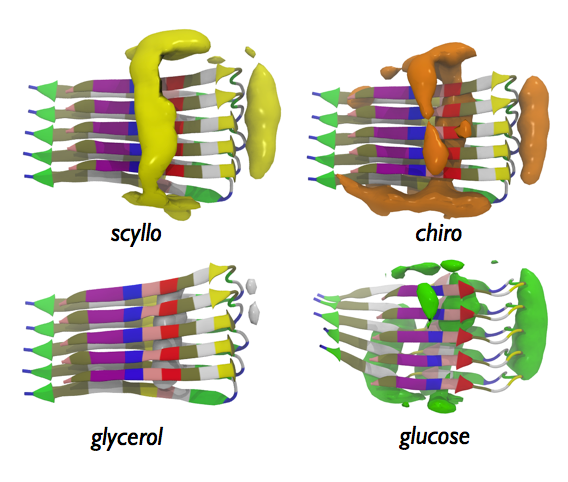
\includegraphics[width=6in]{figures/abeta42_volmaps.png}
  \caption[Abeta42 binding]{Comparisons of global binding for scyllo-, chiro-, glycerol, and glucose}
  \label{fig:spatial_binding}
\end{figure}

\subsection{Comparisons of scyllo, chiro, glycerol and glucose binding}
\begin{itemize*}
	\item The fibril morphology in their presence.  There is only a subtle difference (really? what is this difference? I think I want to retract this statement)
	\item Does glycerol stabilize the aggregate? Does glucose stabilize the fibril?
	\item Is the protofibril equally stable in water and in inositol?
\end{itemize*}

\subsubsection{Inositol and cosolvent Binding} % (fold)
\label{sub:subsection_name}
\begin{itemize*}

	\item Global binding
	\begin{itemize}
		\item Spatial distribution of bound inositol
		\item From a single spatial distribution density for scyllo and chiro-inositol, chiro-inositol bound and passed through the intersheet channel in the fibril, where as scyllo appear to be trapped at the entrance and does not move through the \"channel\". Note that a recent paper by Shea et al. also demonstrated this with dye molecules.	
		\item Contact map -- needed? Yes I think I should further quantitate their binding mode differences. Just by looking at the spatial maps, the differences are minor and need a trained eye.  Having a contact map by residue will be more rigorous. Also quantitate binding affinity per binding pocket. This helps define binding sites on the fibril more precisely. Overall I have more binding statistics than all of the other relevant studies out there, I should take advantage of this. The global binding modes suggests that the active ligand, scyllo-inositol is able to bind the KLVFFAE face better. I need to relate this to fibril inhibition. Furthermore, all of my models are converging on similar answers (that is binding to protofibrils, and binding to KLVFFAE segment), which is reassuring!
	\end{itemize}

	\item Does inositol, glucose and glycerol, preferentially partition to different areas of the protofibrillar surface? Based on the global binding mode as shown in the spatial distribution, the answer to this is yes. But it would be really cool to know the nonpolar and polar binding modes for each of these (that is the pie charts). If there is a difference, I can then extrapolate and correlate these differences to the SAR of inositol.
	
	\begin{itemize}
		\item Nonpolar contacts 
		\item Polar contacts
		\item Binding constants - How do I calculate this?  Inositol never fully dissociates (when saturated) so, in this case, it is more of a residence time in the binding pocket(s). Yes calculate the residence time!  Hmm how do I calculate the residence time? This would link up with the binding kinetics.
	\end{itemize}
\end{itemize*}


\section{Discussion}
Comparisons to earlier simulation studies of inhibitor binding to A$\beta$42 and A$\beta$40 relevance of the NMR models.
``accuracy'' of the NMR models -- how good are these models?  It is unlikely I'm going to be able to say much here, we have no idea what the actual experimental stability of this species is.  This pentamer fragment may not be stable on its own, but could be just a building block in a stable extended fibrillar structure of A$\beta$42.

% look into literature here, read a bit, and critically summarize and fit into the context of my work.
% April 17th 
% Recent papers
% Shea and Bower 2012 in Biochemistry - They looked at CTF binding to Abeta40 and 42 both experimentally and using simulations.  The data here is not that quantitative, esp. the simulation data.  Suggest that N-terminal part of Abeta42 is more responsible for toxicity than the C-termininal.  Also CTF binds at N-terminal (which residues? Don't think this data was in their paper). Does it include 16-22 fragments?
% Abelein et al..Dobson 2012 - Lacmoid binding to Abeta40 and Abeta42.  
% - Proposes a similar mechanism that I am proposing in my KLVFFAE paper .. however they find that Lacmoid most likely binds to the monomer, and in a surfactant-like manner (I think this corresponds to what I call "coating"). 
% - Makes ample references to a paper by Otzen DE http://www.ncbi.nlm.nih.gov/pubmed/20423296 on amyloid aggregation induced by surfactants.  Might be useful to read up on surfactants, micelle formation and what the field knows there.  I can be sure that there will be analogies drawn to this field in my thesis defense.
% - I like what they wrote in the discussion to interpret their data as it somewhat supports my findings, but again speculative and results are STILL pretty qualitative.  
% - Note that this paper might be useful for Aditi to look at ... could she reuse / use some of their protocols?

\subsection{Solute binding}

\begin{itemize}
	\item 	Different binding modes between scyllo and chiro-inositol
	\begin{itemize}
		\item From a single spatial distribution for scyllo and chiro, I did not see scyllo go all the way through the “channel”, where as chiro does! (RESULT)
		\item Is this true in general? Perhaps this is a reason why scyllo works better?  - More specific interactions? ie.  Chiro just gets trapped in ``non-productive'' binding modes.
			\begin{itemize}
				\item Note that Shea also observes this in her paper.\cite{Wu:2011fd}
			\end{itemize}
	\end{itemize}
	\item Sugar binding to the A$\beta$42 fibril -- appears to stabilize? I don't think so … this isn't true from looking at the data.
	
	\item Inositol interestingly also seem to binding similarly to guanidinium ions around a hydrophobic surface. (Personal communication with Shekhar - Said to me during CBP that they see similar results from their guanidinium ion studies ... what does this really mean?)
	
	\item How does binding differ from binding to KLVFFAE, a small fragment of A$\beta$42 ?  Inositol partition differently depending on the sequence. 
	\begin{itemize}
		
		\item Comment on how good are these model peptides for understanding inhibitor binding interactions. Do I really want to discuss this? Depending on the model (the protofibril), the binding modes can be different depending on the aggregate morphology as we've shown in our earlier studies. In our previous study, we examined binding with KLVFFAE.  Because KLVFFAE has identical faces, the preferential binding to KLVFFAE was not identified.  For this reason, we observed that both scyllo and chiro bound with equal Keq to the KLVFFAE.  However, with differing faces, we were able to observe preferential binding to the KLVFFAE face.  This result is consistent with other studies suggesting that targeting this segment of the Abeta is effective in Abeta fibrillation. 
% Binding modes with aggregates consisting of model abeta peptides may have modes that differ from the full length amyloid
		\item Comment on MD simulations as a technique as a whole for understanding these types of interactions
	\end{itemize}
\end{itemize}
 
% - selection targeting to the KLVFFAE face!!!! 
%       - both Joanne and Mark said tonnes of literature supporting this face is relevant for inhibition!!!
%        - so far Scyllo best at binding to this face!! This is an interesting conclusion / difference that thus only could tell from from the abeta42 model because it has two different faces which brought out the preferential binding of Scyllo to this face. 
% 
%         - Regis what if we used Epi or myo a positive control .... Which would make this binding to the KLVFFAE face of abeta42  hypothesis more compelling ... If another inhibitor which worked in vitro also preferentially bound to the KLVFFAE face.

% My attempt to explain why higher affinity for KLVFFAE is a significant result
Many lines of evidence show that KLVFFAE is responsible for fibril formation. (REF: de groot). Targeting the KLVFFAE for inhibition is a promising approach for amyloid inhibition. We hypothesize that binding to the A$\beta$(16-22) face may be a productive small-molecule binding mode for inhibition of lateral stacking of fibrils.  Scyllo- binds this face better than chiro-, glucose, and glycerol inactive solutes in fibril inhibition.  We hypothesize that the difference in their binding affinities to KLVFFAE face explains why scyllo- is active and not chiro-.  Abeta fibrils are less likely to grow as a single layer indefinitely without stacking together.  ie. require stacking to grow into the long unbranched morphology seen in EM. Because KLVFFAE is responsible for stack in fibrils, binding to this face prevents lateral association of fibrillar aggregates and can lead to inhibition of amyloid formation.

% Whole idea:  binding at the surface and preventing stacking, rather than insertion.  Insertion is not likely to be a productive binding mode for inhibition. Why? because I don't observe disruptive insertion (I need to define this) - scyllo doesn't really insert, chiro- does, but no disruption to the aggregate ...
% More quantitatively I probably _need_ to quantify affinity to the KLVFFAE face of the Abeta fibril for scyllo chiro, glucose
% Also should do epi.  But what if epi does not bind to KLVFFAE face? How would I then explain that epi is also active but does not go to KLVFFAE? This could disprove my entire hypothesis ... though its not likely because chiro goes to the KLVFFAE face.
% I think a Shea paper talks about the importance of preventing stacking

\section{Conclusions}
No difference in the fibril conformations with and without inositol in either the low or high molar ratio simulations. Does glucose bind more or less? If it binds less, then it tells us that we might be onto something with scyllo-inositol even though the structure is subtlely different
% Update: glucose does not neccessarily bind ``less", but it does not bind on the right face ie. the KLVFFAE face
Scyllo-inositol appears to preferentially bind the KLVFFAE face, more than glucose and chiro-inositol.  Furthermore scyllo does not bind in a hydrated tunnel formed in the protofibrillar aggregate.

% \acknowledgement
% We thank Drs. JoAnne McLaurin, Mark Nitz and Chris Neale for reading the manuscript and for providing insightful comments. 
% This work was made possible by the GPC supercomputer at the SciNet HPC Consortium and Compute/Calcul Canada (Colosse CLUMEQ). This work was supported in parts by the Canadian Institutes of Health Research (Grant No. MOP84496). R.P. is a CRCP chairholder.

% \section*{Supporting Information Available}
% Binding mode analyses of inositol with monomeric and aggregate systems at inositol concentrations and inositol:peptide molar ratios that were not shown in the main text; Analyses of peptide self-aggregation for the formation of the disordered oligomer; Snapshots of the starting simulation structure of the $\beta$-oligomer. Supporting Information Available: Full description of the material. This material is available free of charge via the Internet at http://pubs.acs.org.

% http://www.pnas.org/content/102/2/315.full
% Support for the Significance of the LVFFA binding:
% The central hydrophobic cluster of amyloid-β (residues 17–21 LVFFA) has been particularly implicated in amyloid fibril formation (19). Tjernberg et al. (20) found that the fragment QKLVFF binds to amyloid β to prevent amyloidogenesis, whereas follow-up studies investigated the short peptides, LVFFA (21) and LPFFD (22), and showed that they are also inhibitors and that the fragment KLVFFAE forms well ordered fibrils. 

% KLVFFA binds to ABeta42 -- do they where they bind?
% Tjernberg, L. O., Naslund, J., Lindqvist, F., Iohansson, J., Karlstrom, A. R., Thyberg, J., Terenius, L., and Nordstedt, C. (1996) Arrest of ������-amyloid fibril formation by a pentapeptide ligand, J. Biol. Chem. 271, 8545-8548.


% Second, Aβ(16-22) peptide, which includes the central HP core, CHC (LVFFA), is recognized as being essential for Aβ fibrillation (27,28) and also forms amyloid fibrils with antiparallel β-strands in isolation (29). Third, the KLVFF motif is a primary target in the search for aggregation inhibitors for AD therapeutics (30,31).
% 28. Nilsberth C., Westlind-Danielsson A., Lannfelt L. The ‘Arctic’ APP mutation (E693G) causes Alzheimer's disease by enhanced Aβ protofibril formation. Nat. Neurosci. 2001;4:887–893. [PubMed]
% 29. Balbach J.J., Ishii Y., Tycko R. Amyloid fibril formation by A β 16-22, a seven-residue fragment of the Alzheimer's β-amyloid peptide, and structural characterization by solid state NMR. Biochemistry. 2000;39:13748–13759. [PubMed]
% 30. Lowe T.L., Strzelec A., Murphy R.M. Structure-function relationships for inhibitors of β-amyloid toxicity containing the recognition sequence KLVFF. Biochemistry. 2001;40:7882–7889. [PubMed]
% 31. Lashuel H.A., Hartley D.M., Callaway D.J. New class of inhibitors of amyloid-β fibril formation. Implications for the mechanism of pathogenesis in Alzheimer's disease. J. Biol. Chem. 2002;277:42881–42890. [PubMed]

\bibliography{shorttitles,ab}
